\chapter{Enfoque de solución}

En el capítulo se pretende hacer alusión a las cuestiones relacionadas con la propuesta de software que se ofrece, brindando definiciones, conceptos, gráficos y demás aspectos que se hagan necesarios para lograr una adecuada comprensión de la implementación realizada.

Se ofrece una solución lo más simple posible, pero que a la vez cubra todas las necesidades y pueda manejar de la manera más adecuada todos los casos de uso que se presenten. Para el desarrollo de la aplicación se emplea un enfoque DDD (Domain Driven Design) y el uso del patrón CQRS (Command and Query Responsability Segregation); en el próximo capítulo (\ref{cap:implementation_details}) se ofrecerá una descripción detallada de tales conceptos así como la razón de la elección.

Si se decidiera describir el sistema en pocas palabras (figura \ref{fig:horario}), se pudiera decir que el horario es una colección de turnos de clase y que un turno de clase está asociado a: un profesor, un local, una asignatura, un grupo, una fecha y un tipo (conferencia, clase práctica, laboratorio, etc); además de cada uno de estos elementos tiene sus propios atributos y relaciones entre ellos. Cada profesor puede definir restricciones sobre el sistema y el cumplimiento (o no de estas) se refleja en la felicidad del horario.

\begin{figure}[h!]
	\centering
	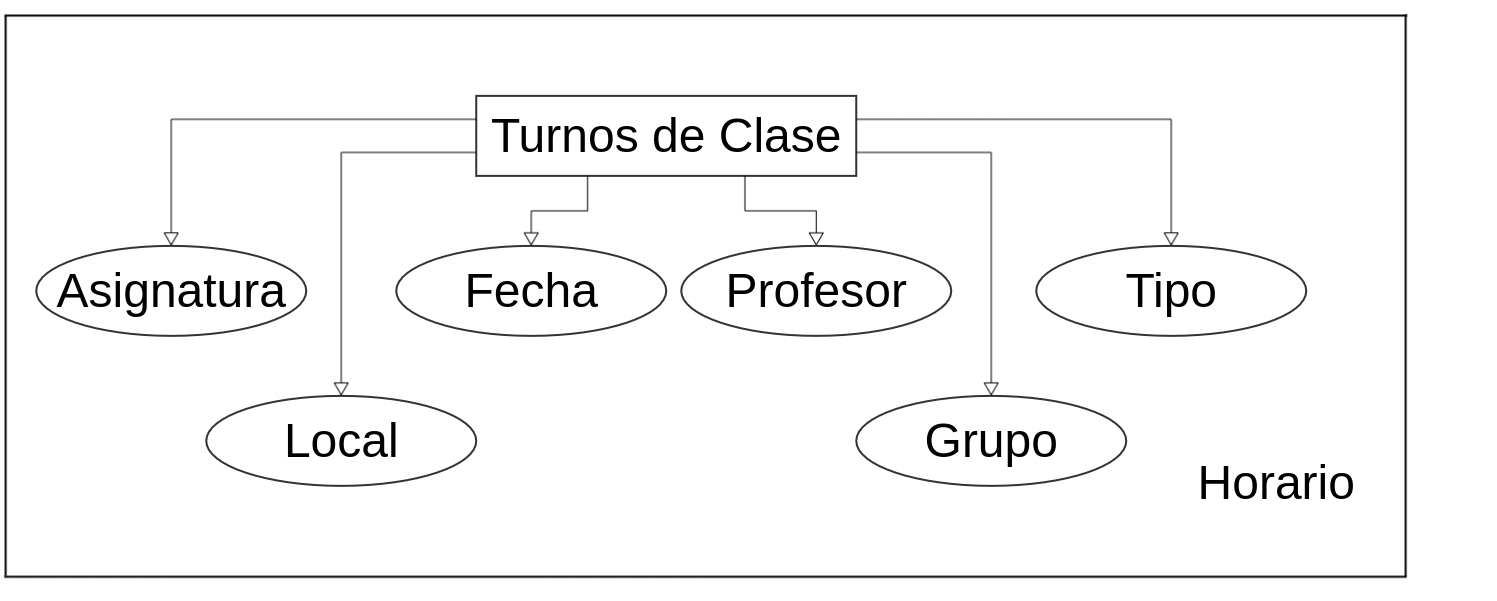
\includegraphics[width=1\linewidth]{images/Chapter 2/horario}
	\caption{Representación del horario}
	\label{fig:horario}
\end{figure}

El uso de esta herramienta y del sistema de horarios en general necesita de un fujo de trabajo que permita en cada momento contar con los datos necesarios para efectuar los pasos correspondientes.

\begin{itemize}
	\item Introducción de los datos administrativos: se actualiza el listado de profesores, locales, asignaturas, grupos, facultades y universidades.
	\item Definición de prioridades dentro de los profesores: a la hora de crear un profesor(o en la edición de este) se hace posible agregar(modificar) el entero que representa la prioridad del mismo. Por defecto la prioridad de un profesor se fija en 1.
	\item Definición de restricciones: los profesores o el administrador del sistema, pueden agregar condiciones sobre la distribución del horario. Para cada restricción además se define la prioridad que tiene. 
	\item Generación de reportes: obtención de un archivo en formato \textit{Excel} que haga posible la distribución del sistema y la posible visualización del mismo de manera offline.
	\item Gestión de semestres y semanas: habilidad de definir los semestres, dígase fecha de inicio y finalización del mismo. Las semanas se crean de forma automática una vez definido el semestre.
	\item Visualización en diversas modalidades: posibilidad de obtener vistas agrupadas por diferentes condiciones; dígase: vistas diarias, semanales, mensuales y por recursos.
	\item Modificación, eliminación y edición de los turnos de clase: tarea principal del sistema.
\end{itemize}

\section{Entidades del sistema}
\label{sec:entities}

Para lograr una mayor comprensión y garantizar por tanto que sea entendido el proceso de modelación del problema; se hace necesario presentar, en primera instancia, una descripción de cada una de las entidades que se usan, así como breves datos de utilidad acerca de estas.

\textbf{Universidad}: Garantizar que el software presentado sea capaz de funcionar en el mayor número de escenarios. Esta entidad es considerada la raíz, en el grafo que representa la relaciones entre todas; es decir, para describir cualquier gestión o para proceder a la confección del horario se hace necesario la previa definición de la universidad. Es válido notar, que en la mayoría de los casos se manejará solamente  una universidad.

\textbf{Facultad}: Maneja todas las facultades presentes dentro de la universidad. La facultad es la encargada de manejar las carreras, así como los locales del sistema. Cada departamento está asociado a una facultad.

\textbf{Carrera}: Agrupa todas las carreras que puedan existir dentro de una facultad. Ofrece una forma de manejar además conjuntos de grupos, profesores y asignaturas.

\textbf{Departamento}: Es la forma más general de agrupar los conjuntos de profesores. Cada departamento pertenece además a una facultad específica.

\begin{figure}[h!]
	\centering
	
\includegraphics[width=1\linewidth]{images/Chapter 3/univ_fac_carr_dep.png}
	\caption{Relación entre Universidad, Facultad, Carrera y Departamento}
	\label{fig:department_relation}
\end{figure}

\textbf{Asignatura}: Constituye uno de los elementos principales del turno de clase, quién es en definitiva la entidad principal del sistema. Las asignaturas se muestran agrupadas por carreras. Además de cada asignatura se conoce el profesor principal que la imparte.

\textbf{Grupos}: Entidad que se encarga de encapsular conjuntos de estudiantes. Mantiene una relación directa con turno de clase, así como con carrera. 

\textbf{Semestre}: Define los diferentes semestres que hay en el sistema. La entidad se llama “semestre” por convención, pero es configurable la cantidad de semanas de duración, mediante una fecha de inicio y una fecha de culminación. En cada semestre se pueden estar gestionando un horario diferente. La idea es que cada usuario del sistema tenga acceso al horario del semestre actual, y que el horario del próximo semestre se pueda ir generando simulatáneamente. Cada semestre está compuesto por varias semanas.

\textbf{Semana}: Esta entidad define y se asocia con una semana del año. Cada semana está contenida dentro de un semestre. Las semanas son generadas automáticamente a partir de la definición del semestre.

\textbf{Tipo de actividad}: Cada uno de los turnos de clase tiene un tipo que resulta importante sobre todo
 para determinar que tipo de aula se necesita. Los tipos más comunes son las conferencias y las clases
 prácticas. Aunque en algunas ocasiones se puede definir además actividades de tipo laboratorio. Es posible generar tipos de actividades nuevas, en caso de que se considere necesario.

\textbf{Local}: Elemento importante que posibilita conocer el lugar donde se impartirá el turno de clase. Es, junto a asignatura y profesor, uno de los elementos principales de un turno de clase. Por lo general a todos los turnos de clases se les asignará un local. En nuestras universidades existen diferentes tipos de locales: salones de conferencia, aulas, laboratorios, anfiteatros, etc. En este sistema los locales se modelaron pertenecientes a una facultad. Cada uno de los locales se define a partir de un “tipo de local” y esta información es utilizada en algunos de los algoritmos que se encargan del manejo de las restricciones.

\textbf{Profesores}: Es una de las entidades de mayor importancia dentro del sistema. Ofrece una vía para asegurar el manejo de todo lo referente a los profesores del centro. Son considerados usuarios especiales o de más relevancia, pues pueden interactuar directamente con el sistema de horarios, imponiendo restricciones o condiciones sobre el mismo. Todos los profesores están agrupados por departamentos. Además cada profesor, puede establecerse como responsable de una asignatura y es posible definir prioridades sobre estos.

\begin{figure}[h!]
	\centering
	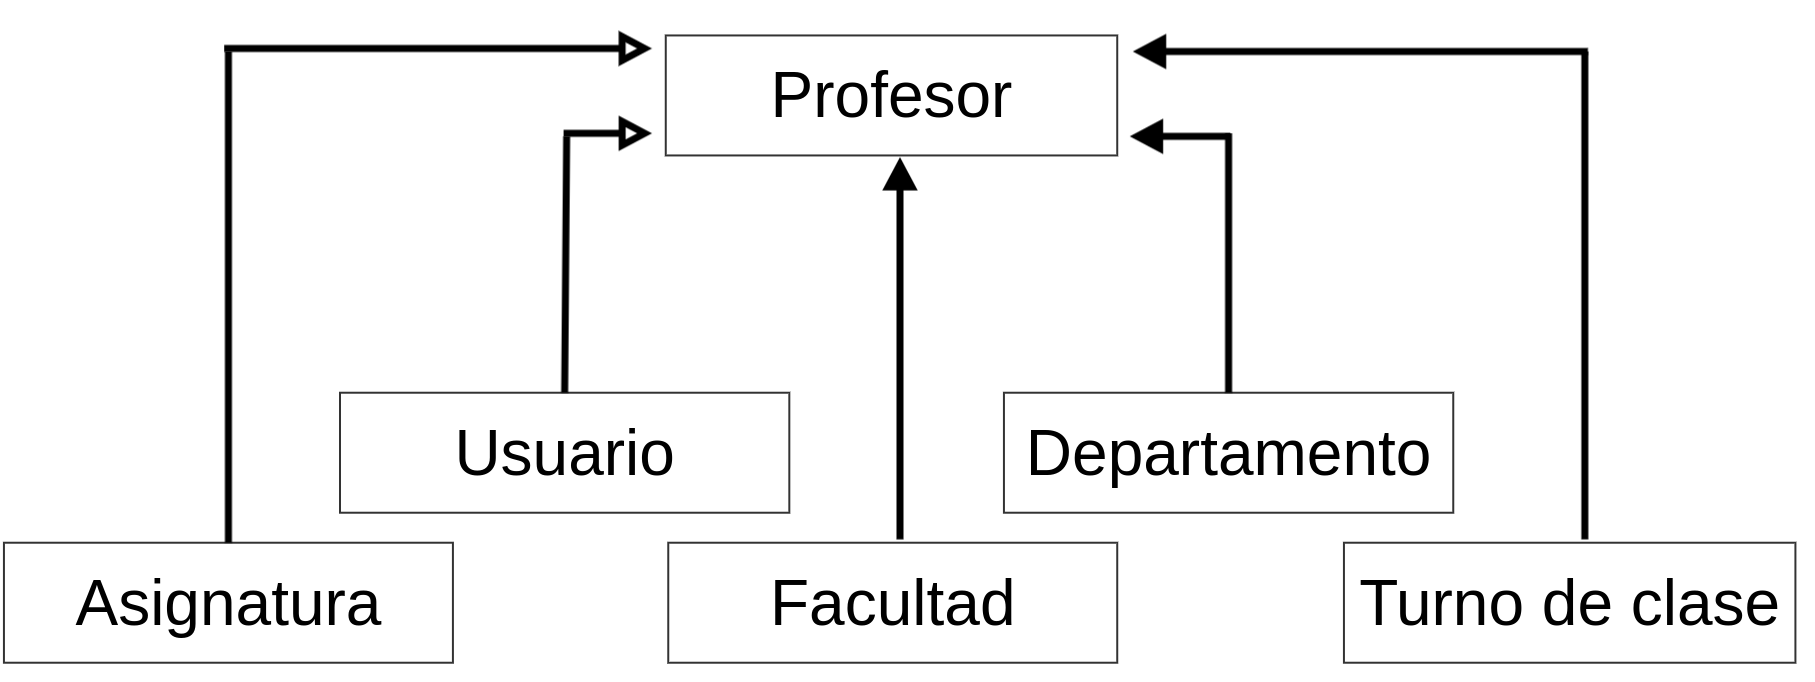
\includegraphics[width=0.75\linewidth]{images/Chapter 2/teacher_relation}
	\caption{Relación entre entidades}
	\label{fig:teacher_relation}
\end{figure}

\textbf{Turno de clase}: Es la entidad fundamental del sistema. Maneja todo lo relacionado con las lecciones que se impartirán en cada uno de los días del semestre, por su imporancia se dedicará la sección \ref{sec:classes} al tratamiento de esta en específico.

\textbf{Restricciones}: Entidad que se encarga de manejar las restricciones o condiciones que los profesores y administradores del sistema pudieran imponer sobre el horario. Las restricciones se describen por medio de varios modelos, uno por cada tipo de restricción manejada. Más adelante se dedicará una sección a la descripción detallada de cada uno de los tipos de restricciones manejadas.

\textbf{Usuarios}: Se encarga de gestionar todo lo referente a los usuarios dentro de la aplicación. Está permitido que cualquier usuario realice registro dentro de la misma, pero solamente el administrador del sistema puede determinar cuáles usuarios son profesores y por tanto, que posean un permiso específico de creación de restricciones. Para un usuario registrado sin permisos, solo es posible la visualización del sistema, cerrando toda forma de modificación o creación de nuevas entidades dentro del mismo. Un usuario puede estar relacionado, a lo sumo, con un profesor. 

\textbf{Reportes}: Módulo que posibilita la obtención de un documento en formato \textit{Excel} que puede ser útil para la posterior distribución del horario, o para la revisión del mismo de manera offline. El documento presenta una serie de páginas: una por cada grupo descrito en el horario y una extra que maneja una representación por locales, es decir, la disponibilidad de los mismos durante todo el semestre. En cada página se encuentra descrito el horario por semanas físicas y además se ofrece una leyenda con la descripción de los turnos de clase así como la hora de comienzo y finalización de los mismos.\\

Cada entidad posee un conjunto de atributos base; por medio de la herencia se logra plasmar esto a la hora de realizar la implementación. 

Todas las entidades del sistema heredan de \texttt{DomainEntity}, que no es más que una \textit{clase abstracta} con un constructor privado y una definición específica de un método \textit{equals}. Esta clase está descrita además por una serie de propiedades base:

\label{props:base}
\begin{itemize}
	\item \textsl{Nombre completo}: Propiedad de tipo texto que almacena el nombre en formato largo del objeto que se esté referenciando en ese momento. 
	\item \textsl{Nombre reducido}: Propiedad de tipo texto que almacena el nombre en formato corto del objeto que se esté referenciando en ese momento. 
	\item \textsl{Descripción}: Propiedad de tipo texto que contiene detalles, acerca del objeto que se esté referenciando en ese momento. Esta propiedad puede tomar valores nulos.
	\item \textsl{Prioridad}: Propiedad de tipo numérico que almacena la prioridad que pudiera tener un objeto (o entidad) sobre otro, en el sistema. Es utilizada principalemte en el cálculo de la \textit{felicidad del sistema}.

\end{itemize}



\section{Modelo entidad-relación (MERX)}

El siguiente modelo propone describir las relaciones existentes entre todas las entidades presentes en la base de datos. Para confeccionar el mismo se siguen las convenciones de estilo (\ref{sec:style_conventios}), abordadas en el capítulo anterior.


\begin{figure}[h!]
	\centering
	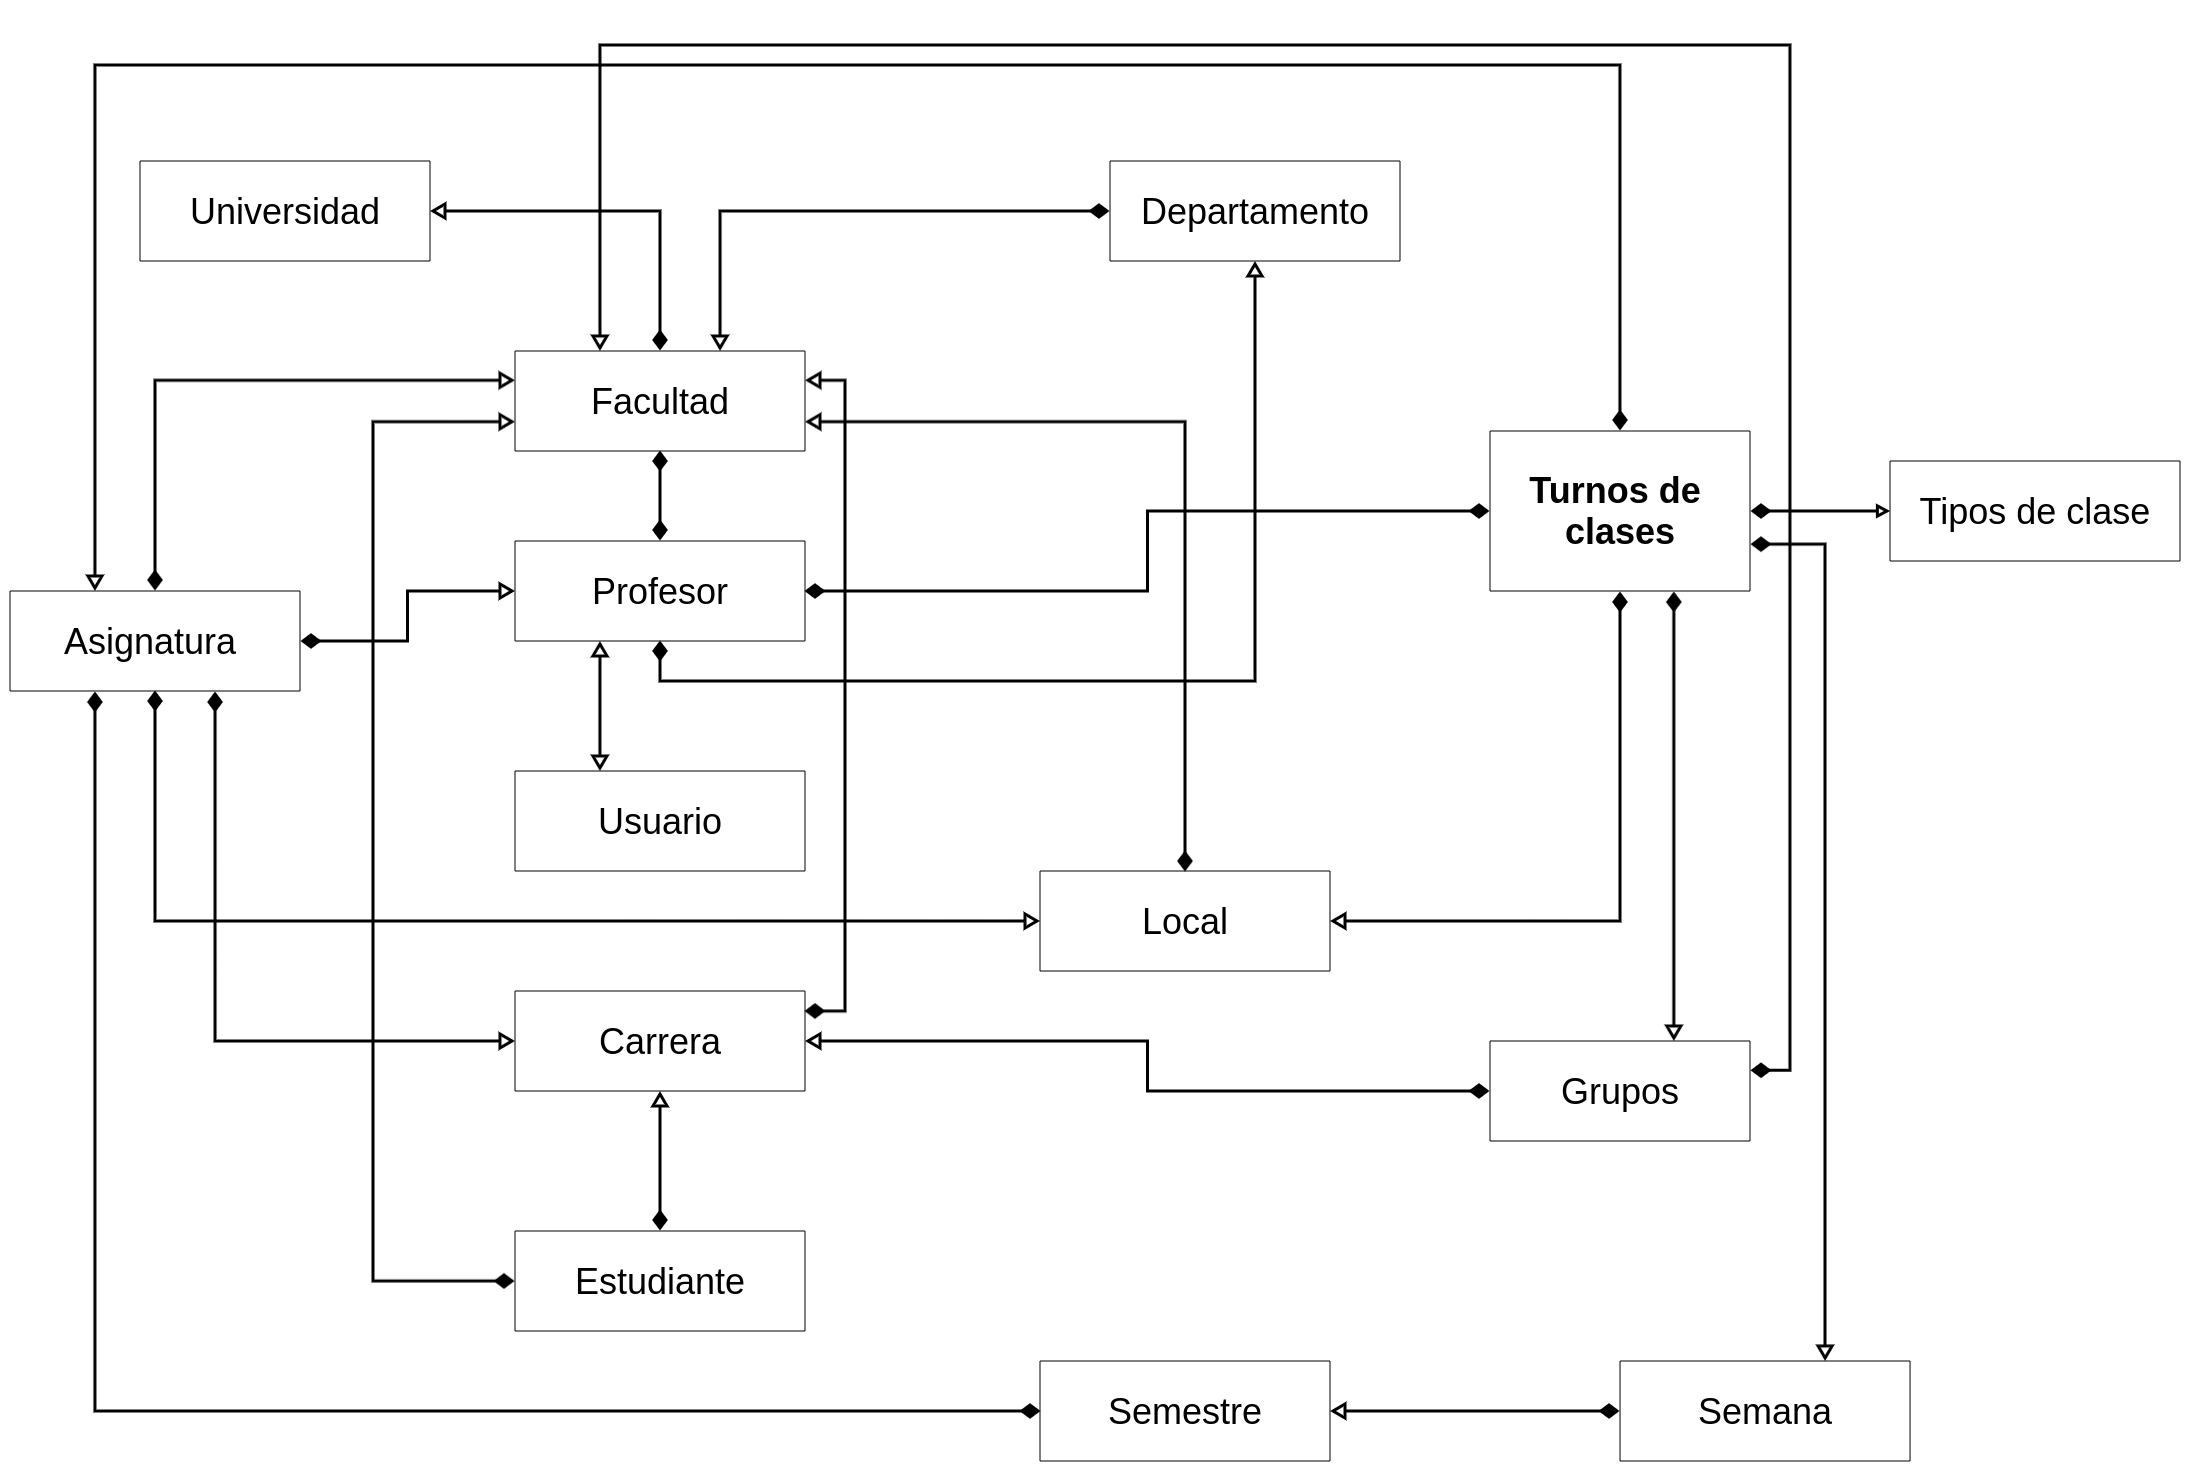
\includegraphics[width=1\linewidth]{images/Chapter 2/MERX}
	\caption{ Modelo entidad-relación }
	\label{fig:merx}
\end{figure}


\section{Turno de Clase}
\label{sec:classes}

El \textit{turno de clases} es la entidad fundamental que compone todo sistema de horarios. Como aspecto común a la mayoría de los turnos de clase (de las universidades cubanas) se tiene que estos cuentan una duración de 90 minutos y que se pueden clasificar en dos tipos básicos: conferencias y clases prácticas.

En la Universidad de La Habana se estila a separar el día en dos secciones: mañana y tarde, y que cada sección esté compuesta por tres turnos de clase. Es válido notar que esto se realiza por una especie de convenio ya preestablecido, pero el sistema cuenta con las herramientas para variar este funcionamiento haciendo posible, por tanto, la modificación de los mismos. 

Un turno de clases está compuesto por los siguientes atributos:
\begin{itemize}
	\item \textit{Atributos base}: definidos en la sección \ref{props:base}
	\item \textit{Inicio}: marca la hora de inicio del turno de clase.
	\item \textit{Finalización}: marca la hora de finalización del turno.
	\item \textit{Id de recurso}: referente al \texttt{id} del local; se utiliza mayormente en el manejo de la vista asociada a los recursos.
	\item \textit{Semana}: referente a la semana en que se impartirá el turno de clase.
	\item \textit{Profesores}: colección de elementos que representan los profesores encargados de impartir las clases; notar que al menos siempre se contará con un profesor responsable, que se toma de la asignatura referente al turno.
	\item \textit{Local}: referente al local donde se impartirá el turno de clase.
	\item \textit{Asignatura}: referente a la asignatura.
	\item \textit{Tipos de clase}: referente al tipo de clase (conferencia, clase práctica, laboratorio).
	\item \textit{Grupo}: referente al grupo.
\end{itemize}

Es común notar que en muchos sistemas de horarios, por no decir en todos, contamos con la misma frecuencia de turnos todas las semanas, o a lo sumo en intervalos de quince días. Para ganar en usabilidad y por tanto mejorar la experiencia de usuario se presenta un enfoque que permite crear turnos en una frecuencia específica; dicho en otras palabras y mostrado a través de un ejemplo: si tenemos, dado el caso, que el turno de Matemática Discreta de 2$^{do}$ de Computación se realiza los martes de todas las semanas, en la aplicación no es necesario recorrer todos los martes del semestre e ir definiéndolos uno por uno. Para ello se ofrece una especie de configuración y el sistema se encarga de la posterior creación de cada uno. Este enfoque se maneja a través del concepto de \textit{turnos en serie}.

\begin{dfn}
	Turnos en serie: habilidad que hace posible la replicación de un turno a través de todo el semestre, para ello hay que contar con la previa definición de la frecuencia del mismo y los días, dentro de la semana, en que se impartirá. El turno replicado tendrá las mismas características que el original, exceptuando las fechas involucradas.
\end{dfn}

El manejo de turnos en serie nos crea una relación entre los mismos, o sea, los turnos de una misma serie están relacionados entre ellos, esto hace posible que la edición y eliminación de cualquier turno de la serie influya también en el resto de estos turnos. Estas operaciones son además flexibles, dado el hecho de que también es posible modificar inidividualmente los turnos de cualquier serie sin afectar al resto. Una vez que turno perteneciente a una serie se modifica individualmente, este turno ya no pertenecerá más a la serie inicial y por tanto cualquier modificación que se le aplique al mismo no repercutirá en nadie más.

El sistema cuenta con una serie de filtros dedicados a obtener secciones del mismo. Los turnos de clase están adaptados, por tanto, a estos requerimientos. Se hace posible agregar filtros por tiempo (día-hora de inicio y finalización), así como por asignaturas, grupos, locales, tipos de clase y facultades.

\section{Manejo de restricciones}
\label{sec:restrictions}

El uso de restricciones es una de las partes más llamativas de este sistema, la idea detrás del manejo e implementación de las mismas surge a través del trabajo de diploma desarrollado por el estudiante \textit{Joel Rey Travieso Sosa} \cite{thesis_joel} perteneciente a la Facultad de Matemática y Computación de La Universidad de La Habana.

El análisis y la gestión de las restricciones trajo consigo la clasificación en diferentes grupos:
\begin{itemize}
	\item \textit{Asignación de recursos}: Cuando un recurso debe ser asignado a otro recurso de distinto tipo o a cierto evento.
	\item \textit{Asignación de tiempo}: Cuando un evento o recurso debe asignarse a una fecha.
	\item \textit{Restricciones de tiempo entre eventos}: Cuando un evento mantiene una relación de tiempo con otro.
	\item \textit{Solapamiento de eventos}: Cuando un grupo de eventos comparte un mismo intervalo de tiempo.
	\item \textit{Coherencia entre eventos}: Intentar producir horarios más organizados y convenientes.
	\item \textit{Capacidad}: Algunos de los recursos tienen capacidades de uso que no pueden ser vulneradas.
	\item \textit{Continuidad}: Cuando se intenta producir horarios con determinadas características constantes o muy predecibles.
	
\end{itemize}

Además se detectaron cinco grupos fundamentales para clasificar las condiciones o requerimientos del problema:
\begin{itemize}
	\item \textit{Restricciones unarias}: aquellas que involucran un sólo evento, como por ejemplo, las clases de un curso no pueden ser programadas un día lunes.
	\item \textit{Restricciones binarias}: aquellas que involucran dos eventos. Un ejemplo típico son las restricciones de topes de horarios para un curso que requiere un mismo recurso: profesor, sala de clases, etc
	\item \textit{Restricciones de capacidad}: las que se imponen al asignar cursos a salas de clase con capacidad suficiente.
	\item \textit{Restricciones de separación de eventos}:  aquellas que requieren que las actividades estén separadas o siguiendo algún patrón en el tiempo. Algunos ejemplos son las impuestas por políticas de la institución de respetar asignaciones de horarios en patrones predefinidos o las condiciones de no existencia de horas intermedias vacías.
	\item \textit{Restricciones asociadas a los  agentes}: las limitaciones en los horarios asignados para cumplir con las preferencias de los profesores.
\end{itemize}

En la implementación que se ofrece se manejan 4 tipos de restricciones fundamentales, que cubren la descripción antes mencionada.
\begin{itemize}
	\item Restricción de requerimiento de cuenta simple.
	\item Restricción de requerimiento de cuenta de condiciones.
	\item Restricción de requerimiento de distribución de atributos.
	\item Restricción de requerimiento relacional.
\end{itemize}

Cada profesor propone un conjunto de condiciones que se aplica a los turnos de clase, además de cada profesor se conoce la prioridad, así como la prioridad particular que le otorga a cada restricción. 
Con el objectivo de expresar un concepto un poco más formal: 
\begin{dfn}[Restricción]
	Forma por medio de la cuál los usuarios (principalmente los profesores) expresan sus consideraciones acerca de los elementos que determinan la calidad de cualquier horario propuesto; ya sea en sentido general o personal.
\end{dfn} 

Cada restricción cuenta con un grupo de elementos comunes (figura \ref{fig:base_restrictions}):\\

\paragraph{Condiciones.}
Permite identificar a qué turnos se exigirán determinados requerimientos. Define el filtro inicial que se impone sobre el conjunto de turnos, para obtener así un subconjunto de los mismos, los cuáles deberán cumplir estrictamente los requisitos planteados.\\
	
Una condición está compuesta por un atributo \texttt{A}, y en función de este, un operador \texttt{O} y un valor \texttt{V}. Un atributo relativo a un turno puede ser en realidad, un atributo relativo a una entidad asociada al turno de clase.\\

\begin{table}[h]
	\centering
	\begin{tabular}[c]{l|l|l|r}
		\textbf{Ejemplo}                   & \textbf{Atributo}     & \textbf{Operador} & \textbf{Valor} \\ 
		\hline 
		Aula con más de 30 alumnos         &  Capacidad del Local  & >                 & 30             \\ 
		Ser un martes					   & Día del Turno         & ==                & martes
	\end{tabular}
	\caption{Ejemplos de representación de condiciones}
	\label{tab:conditions}		
\end{table}

Es posible también garantizar el manejo de grupos de condiciones para asegurar que se puedan formular la totalidad de las operaciones deseadas.

\begin{dfn}[Grupo de condiciones]
	Forma amigable de representar un bloque de condiciones lógicas encerradas entre paréntesis; y asegurar, por tanto, la manera correcta de evaluación del mismo. El conjunto de condiciones de una restricción puede verse como un grupo de condiciones.
\end{dfn}

Ejemplos de grupos de condiciones: 
\begin{itemize}
	\item "Ser lunes". Una condición que involucra un solo operador lógico también es considerado un grupo de condiciones.
	\item (Turnos de Matemática Discreta) (del martes). 
	\item (Turnos de Matemática Discreta o de Matemática Numérica) (del martes).
\end{itemize}

\paragraph{Intervalo.}
Ofrece una forma de obtener una separación del  conjunto de turnos en subconjuntos, cada uno conteniendo los turnos correspondientes a un período de tiempo diferente, en cada caso de tamaño \textit{intervalo}, salvo quizás, el último, en caso de que el curso no pueda ser dividido exactamente en un número 
entero de intervalos de tamaño \textit{intervalo}. El objetivo detrás de esta separación del conjuto de turnos en intervalos, en segregar aún más la evaluación; pues, por ejemplo, supogamos que estamos analizando una restricción sobre $X$ y que: $\exists y \in X $ tal que para $y$ la restricción se incumple, entonces resultaría un poco antiintuitivo decir que la restricción se incumple, solo porque fallara en un turno, por ello si consideramos que $intervalo = 7$ (análisis semanal), entonces el turno entraría solo en una semana de las analizadas y por tanto la restricción no se inclumpliría en su totalidad, lo que influiría positivamente en la felicidad del sistema.

\paragraph{Prioridad.}
\label{def:priority}
Establece la prioridad de la restricción. El usuario creador de la restricción (profesor o administrador del sistema) deberá establecer la priridad o cuán importante es la restricción que se está definiendo. Por defecto, si el valor no se proporciona, se fija en 1. Este valor se utilizará posteriormente para el cálculo de la \textit{felicidad} del sistema. La utilidad del mismo radica en gestionar de alguna manera una especie de jerarquía y posibilitar, por tanto, un orden para lograr ser lo más semenjante posible a la vida real.

\paragraph{Descripción.}
Este campo se presenta de manera obligatoria a la hora de la creación de nuevas restricciones. Es un forma de representar con palabras lo que se pretende crear y hacer posible por tanto la rápida comprensión e interpretación de la misma. 

\paragraph{Profesor.}
Se emplea para referenciar al profesor al que está destinada la restricción. En cada de que la restricción sea creada por el profesor en sí, y no por el administrador del sistema, el valor del campo se fijará automáticamente. \\\\

El conjuto de campos definidos por cada tipo de restricción varía en dependencia del tipo.

\begin{figure}[h]
	\centering
	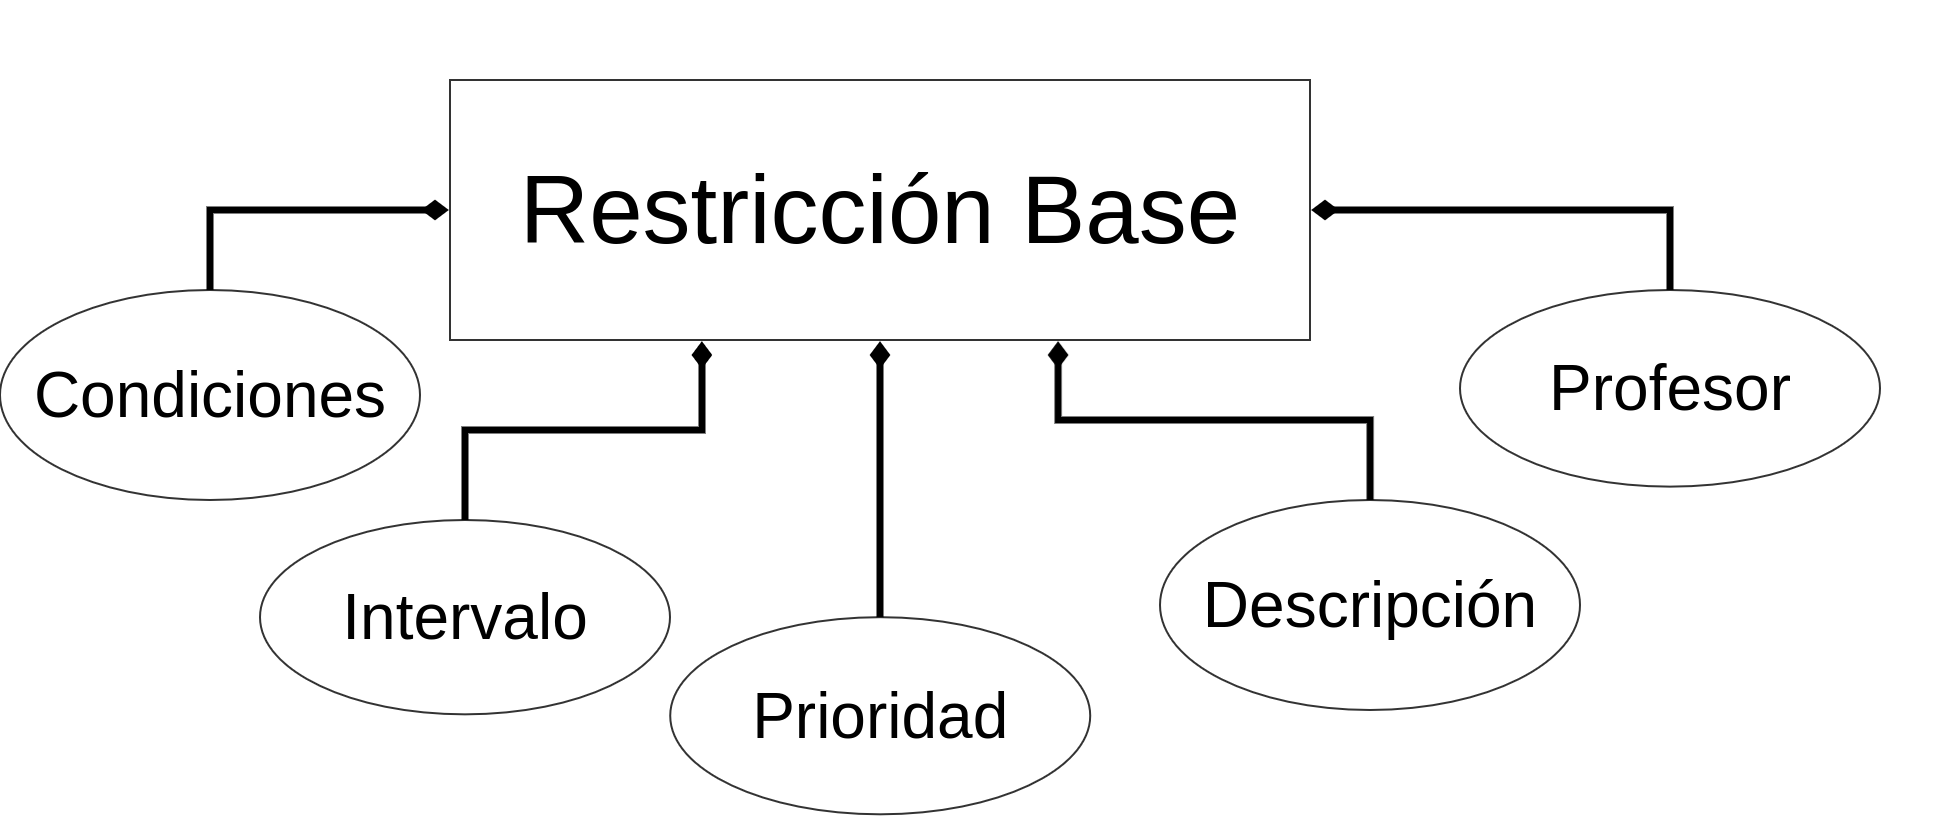
\includegraphics[width=0.75\linewidth]{images/Chapter 2/base_restrictions}
	\caption{Restricción base.}
	\label{fig:base_restrictions}
\end{figure}

\subsection{Tipos de restricciones}

Es posible manejar o declarar diversos timpos de restricciones, dichos tipos ya fueron enunciados en las secciones previas (\ref{sec:restrictions}) de este documento.

\paragraph{Restricción de requerimiento de cuenta simple.}  Esta restricción se refiere al número de turnos que han satisfecho las condiciones fijadas inicialmente. El usuario debe configurar el operador de comparación \textit{O} a aplicar y el valor \textit{V} con el cual comparar. La restricción se cumple si la cantidad de turnos que satisfacen las condiciones mantiene una relación \textit{O} con \textit{V}. El valor de \textit{V} puede ser numérico, porcentual o bien fraccionario  con respecto al total de turnos que pasan la etapa de las condiciones.
 
Referente a este tipo de restricción se puede tomar como ejemplo: todos los turnos de Matemática Numérica de 3$^{ro}$CC deben realizarse los lunes. 
 

\paragraph{Restricción de requerimiento de cuenta de condiciones.} Este requerimiento se refiere a qué parte del conjunto de turnos que ha satisfecho las condiciones previas, cumple también un bloque de condiciones adicionales, y cuenta además con el operador de comparación \textit{O} a aplicar y el valor \textit{V} con el cual comparar. El requerimiento se cumple si la cantidad de turnos que satisfacen las condiciones iniciales y satisfacen simultáneamente otras que se han configurado, mantiene una relación \textit{O} con \textit{V}.

Como ejemplo de este tipo de restricción se puede considerar: todos los turnos de Matemática Discreta de CC tienen que ser lunes o viernes.

\paragraph{Restricción de requerimiento de distribución de atributos.} Este requerimiento se refiere a la cantidad de valores distintos que puede tomar determinado atributo en el conjunto de turnos que pasa la etapa de condiciones. El usuario configura, además del atributo \textit{A}, el operador de comparación \textit{O} y el valor \textit{V}. El requerimiento se cumple si la cantidad de valores que toma el atributo \textit{A} en el conjunto de turnos que cumple las condiciones previas mantiene una relación \textit{O} con  \textit{V}. En este caso el valor de \textit{V} debe ser numérico.

Un ejemplo mediante el cuál se evidencia esta restricción pudiera ser: el profesor \textit{X} imparte las asignaturas de Sistema Operativo y Redes en CC, pero no se puede dar la situación de que tenga que dar las dos asignaturas en la misma semana; dicho en otras palabras, si en la semana \textit{A} se le ponen turnos de Sistema Operativo, entonces no se le deben asignar turnos de Redes.

\paragraph{Restricción de requerimiento relacional.} Este requerimiento se refiere a la relación que mantiene el conjunto de turnos que cumplen las condiciones previas con otro que cumple otro grupo de condiciones. En este caso se requiere que el usuario añada un segundo grupo de condiciones que filtrarán el segundo conjunto de turnos, un atributo \textit{A} y un operador booleano de conjuntos \textit{O} que define la relación entre los valores de \textit{A} en el primer conjunto y el segundo. El requerimiento se cumple si el conjunto de valores que toma \textit{A} en el primer conjunto de turnos mantiene una relación \textit{O} con el conjunto de valores que toma \textit{A} en el segundo conjunto.

Un ejemplo que describe la restricción puede ser: el profesor \textit{X} imparte clases de las asignaturas de Sistema Operativo y Redes para la carrera de CC, entonces se quiere que de ser posible, las asignaturas se puedan impartir el mismo día; es decir, cada vez que tenga un turno de Sistema Operativo se quiere que también imparta su turno de Redes.


\begin{figure}[h!]
	\centering
	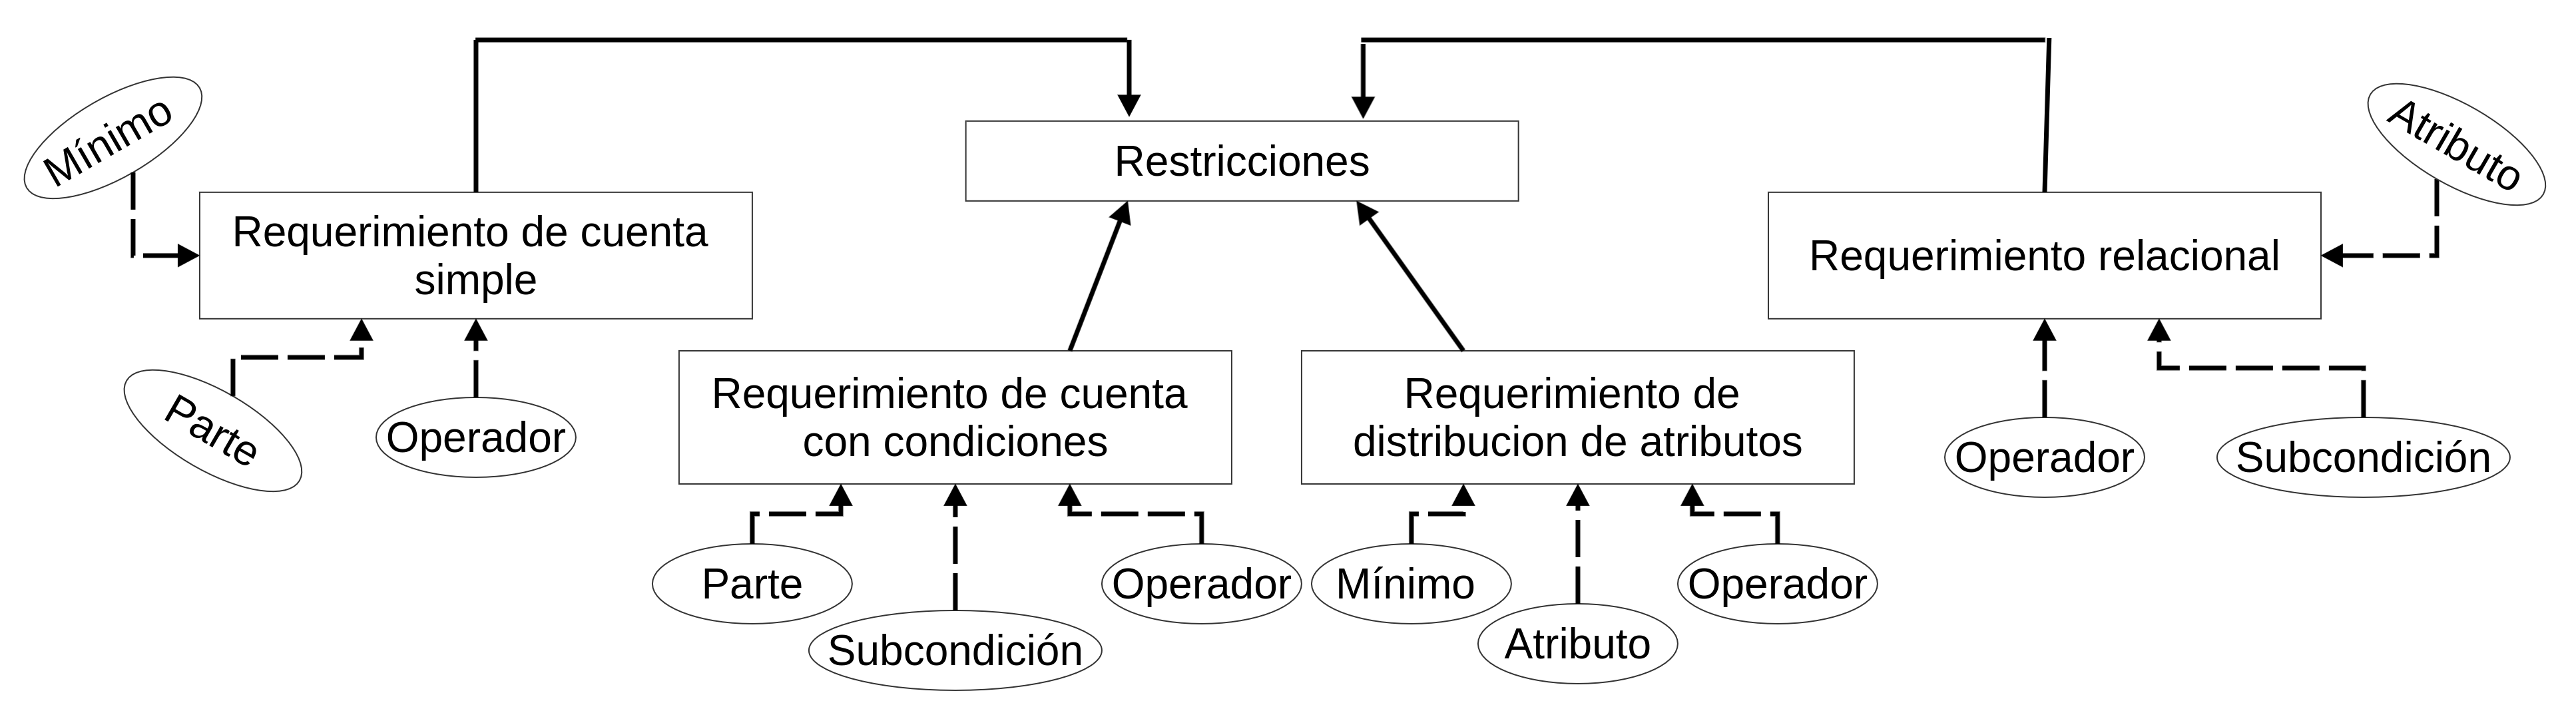
\includegraphics[width=0.95\linewidth]{images/Chapter 2/restrictions}
	\caption{Restricciones con sus atributos.}
	\label{fig:restrictions}
\end{figure}


\section{Felicidad del sistema}
\label{sec:happiness}

La felicidad del sistema, es una cuestión a la que se ha venido haciendo alusión desde los capítulos anteriores. Este valor se obtiene a través de la felicidad relativa a cada uno de los profesores y su posterior procesamiento teniendo en cuenta una fórmula previamente definida.

\begin{dfn} [Felicidad del sistema]
	Valor definido entre 0 y 100 que no es más que un medidor de la calidad del horario.
\end{dfn}

La estrategia utilizada para arribar a las fórmulas de cálculo de felicidad en profesores y en el sistema completo, es básicamente la misma; y se basa en el peso de las prioridades (\ref{def:priority}) establecidas con anterioridad en cada unas de las entidades.

\subsection{Fórmula de la felicidad relativa a un profesor}
Para calcular la felicidad relativa a un profesor con respecto al cumplimiento de sus restricciones, se empleará la siguiente fórmula.

\begin{equation}
	f_p = \frac{w_{1p}c_{1p} + \dots + w_{np}c_{np} }{w_{1p} + \dots + w_{np}}
\end{equation}

\noindent Donde se tiene que: \\

\begin{itemize}
 	\item $w_{ip} \in \mathbb{N}_+ $: Prioridad del requerimiento i-ésimo del profesor p-ésimo
	\item $c_{ip} \in \{0, 1\}$: Cumplimiento del requerimiento i-ésimo del profesor p-ésimo
	\item $n \in \mathbb{N}_+$: Cantidad de requerimientos
	\item $f_p \in [0, 1]$: Felicidad del profesor p-ésimo
\end{itemize}

\subsection{Felicidad relativa al sistema}
Para calcular la felicidad total del sistema se emplea el cómputo de las felicidades respectivas de los profesores:

\begin{equation}
	F_T = \frac{f_1p_1 + \dots + f_mp_m}{p_1 + \dots + p_m}
\end{equation}

\noindent Donde se tiene que:
\begin{itemize}
	\item $f_m \in [0, 1]$: Felicidad del profesor m-ésimo.
	\item $p_m$: Prioridad del profesor m-ésimo.
	\item $m \in \mathbb{N}$: Cantidad de profesores.
\end{itemize}





